\documentclass[10pt,twocolumn,letterpaper]{article}

\usepackage{cvpr}
\usepackage{times}
\usepackage{epsfig}
\usepackage{graphicx}
\usepackage{amsmath}
\usepackage{amssymb}

\cvprfinalcopy

\def\cvprPaperID{****}
\def\httilde{\mbox{\tt\raisebox{-.5ex}{\symbol{126}}}}

% Pages are numbered in submission mode, and unnumbered in camera-ready
\ifcvprfinal\pagestyle{empty}\fi
\begin{document}

%%%%%%%%% TITLE
\title{M5 Forecasting - Accuracy: Estimate the unit sales of Walmart retail goods}

\author{Flavio Amurrio-Moya\\
George Mason University\\
4400 University Dr, Fairfax, VA 22030\\
{\tt\small famurrio@gmu.edu}
\and
Pyoung Kang Kim\\
George Mason University\\
4400 University Dr, Fairfax, VA 22030\\
{\tt\small pkim23@gmu.edu}
}

\maketitle
\thispagestyle{empty}

%%%%%%%%% ABSTRACT
\begin{abstract}
% Problem, gap, approach, key results
  Methods based on decision trees dominate the field of tabular regressional
  problems and have shown to outperform many other methods such as weighted
  averaging and other statistical methods and even outperforming methods that
  are natively time series based on using networks such as LSTM/GRU. In this
  report, we plan to test out a pure Deep Learning approach which leverages key
  foundation concepts in both supervised and unsupervised learning to attempt to
  reach an acceptable score with minimum data manipulation, and virtually no
  data gathering/wrangling.

  The ``M5 Forecasting - Accuracy: Estimate the unit sales of Walmart retail
  goods'' competition (will be referred to as the ``M5 Forecasting Competition''
  and ``The Competition'') challenged Kaggle users to design a learning model
  that would be able to predict how many of a certain item would be sold on a
  given day. In this paper, we embark in the challenge to create such a model
  and improve on current strategies.

\end{abstract}

%%%%%%%%% BODY TEXT
\section{Introduction}
% Broad problem and impact
% scientific gap(what technical aspects have not yet been solved)
% summary approach (should include reference to technical gap)
% key results
The M5 Forecasting competition was created on Kaggle by ``The Makridakis Open
Forecasting Center (MOFC) at the University of Nicosia''. This was done with the
intent of being able to forecast the sales of items in order to minimize
opportunity loss (such as not having enough of an item in stock) as well as to
avoid stocking too much of an unpopular item. This competition aims to achieve
more accurate and better-calibrated forecasts, reduce waste and be able to
appreciate uncertainty and its risk implications.

In this paper, we discuss an approach to tabular regressional learning that is
an end to end Deep Learning solution. We try various modifications to the
network and it's loss function and discuss key points that will help achieve
higher scores on the Competition.

We were provided with hierarchical sales data from Walmart to forecast daily
sales for the next 28 days. The data covers stores in three US states
(California, Texas, and Wisconsin) and includes item level, department, product
categories, and store details. It also contains explanatory variables such as
price, promotions, day of the week, and special events.



\subsection{Data}
  We were given a star schema dataset of csv files that contained 3 files to be
  used for training.

  calendar.csv - information regarding dates of product sales.

  schema - date, wm\_yr\_wk, weekday, wday, month, year, d, event\_name\_1,
  event\_type\_1, event\_name\_2, event\_type\_2, snap\_CA, snap\_TX, snap\_WI

  row - 2011-01-29, 11101, Saturday, 1, 1, 2011, d\_1, , , , , 0 , 0 , 0


  sales\_train\_validation.csv - actual sales respective to date ‘d’, by hierarchical data
  schema - id, item\_id, dept\_id, cat\_id, store\_id, state\_id, d\_1, ...d\_1913

  row - HOBBIES\_1\_001\_CA\_1\_validation, HOBBIES\_1\_001, HOBBIES\_1, HOBBIES, CA\_1, CA, 0, ...1

  sell\_prices.csv - prices of products per a certain store and date

  schema -  store\_id, item\_id, wm\_yr\_wk, sell\_price

  row - CA\_1, HOBBIES\_1\_001, 11325, 9.58



\subsection{Closer Look At The Data}


\begin{figure*}
  \begin{center}
    % \fbox{\rule{0pt}{2in} \rule{.9\linewidth}{0pt}}
    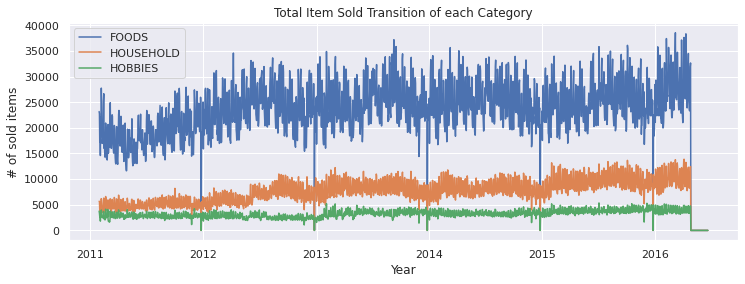
\includegraphics[width=0.8\linewidth]{img/totalItemSoldofEachCategory.png}
  \end{center}
  \caption{Total items sold of each category.}
  \label{fig:totalItemSoldofEachCategory}
\end{figure*}
In Figure~\ref{fig:totalItemSoldofEachCategory} shows ...

\begin{figure*}
  \begin{center}
    % \fbox{\rule{0pt}{2in} \rule{.9\linewidth}{0pt}}
    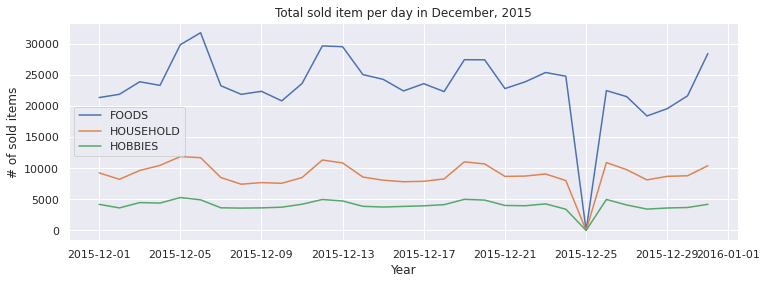
\includegraphics[width=0.8\linewidth]{img/totalSoldItemPerDayDec2015.png}
  \end{center}
    \caption{Total items sold per day in December 2015.}
  \label{fig:totalSoldItemPerDayDec2015}
\end{figure*}
In Figure~\ref{fig:totalSoldItemPerDayDec2015} shows ...


\begin{figure*}
  \begin{center}
    % \fbox{\rule{0pt}{2in} \rule{.9\linewidth}{0pt}}
    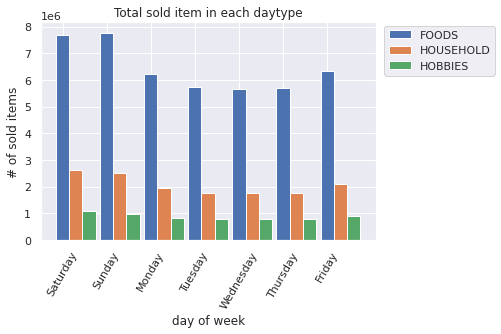
\includegraphics[width=0.8\linewidth]{img/totalSoldItemInEachDayOfWeek.png}
  \end{center}
    \caption{Total items sold each day of the week}
  \label{fig:totalSoldItemInEachDayOfWeek}
\end{figure*}
In Figure~\ref{fig:totalSoldItemInEachDayOfWeek} shows ...


\begin{figure*}
  \begin{center}
    % \fbox{\rule{0pt}{2in} \rule{.9\linewidth}{0pt}}
    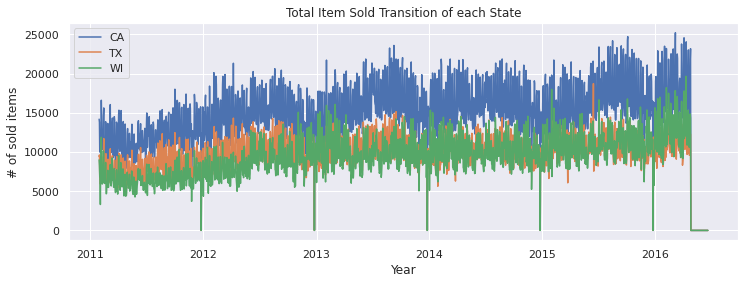
\includegraphics[width=0.8\linewidth]{img/totalItemSoldInEachState.png}
  \end{center}
    \caption{Total items sold in each state.}
  \label{fig:totalItemSoldInEachState}
\end{figure*}
In Figure~\ref{fig:totalItemSoldInEachState} shows ...





%-------------------------------------------------------------------------
\section{Approach}
% Background tutorial (if necessary)
% Your technical innovation (might be multiple pages/sections, with repeated reference to scientific gap)
  The approach corresponds with the files attached to the BlackBoard submission,
  which contains all the source code used to generate files, train, and run
  evaluation on.

\subsection{Dataset}
In order to train a Neural Network that can learn to correctly predict the
number of sales per the hierarchical data shown above, i.e. item in a
department, in a particular store, in a particular state, for a particular range
of dates, we collapsed the star schema into a singular table containing all this
particular information, with the dates and corresponding sales both becoming
respondent columns. The training file ended up looking as such.

sales.csv - training file for the neural network, containing labels and its
respective metadata. 

\noindent schema - sales, id, item\_id, dept\_id, cat\_id, store\_id, state\_id, d, date, wm\_yr\_wk, weekday, wday, month, year, event\_name\_1, event\_type\_1, event\_name\_2, event\_type\_2, snap\_CA, snap\_TX, snap\_WI, sell\_price

 \noindent row: 0, HOBBIES\_1\_001\_CA\_1\_validation, HOBBIES\_1\_001, HOBBIES\_1, HOBBIES, CA\_1, CA, d\_1, 2011-01-29, 11101, Saturday, 1, 1, 2011, , , , , 0, 0, 0,

The column sales correspond to the number of products sold at that certain date
per the hierarchical item. In order to develop such a training set, it is
necessary to check for the correctness of the data. We made sure there are no
duplicate columns/rows, and that all data was filled correctly for a correct
merge operation between the respective fields across the tables. All the joins
were done using outer joins, so come resulting rows had missing fields such as a
pricing per item at a particular date

 The sales\_train\_validation.csv contained 30490 entries, however, with the
sales.csv having rolled out the dates into columns of their own, and having
merged with its surrounding tables, it became over 60 million rows, a job for a
server computer with at least 50gb of ram. At the time, we didn’t have access to
a server computer, thus partitioned data and then finally concatenated them
together. Once we had access to a server computer with 128gb of ram, we were
able to load the dataset into memory. Loading the file into a pandas dataframe
took over 4 minutes. However, after manually typing the pandas’ columns to
smaller data types, the load took somewhere around 3-4 minutes. The type was
defined as below.

 'snap\_CA': 'int8', 'snap\_TX': 'int8', 'snap\_WI': 'int8', 'sales': 'float32',
 'wm\_yr\_wk': 'int16', 'wday': 'int8', 'month': 'int8', 'year': 'int8',
 'sell\_price': 'float32'

\subsection{Model/Data}
The model we used was a tabular model from a popular repository on GitHub,
https://github.com/fastai/fastai. The underlying details worked as so. We
defined the dataset to be fed to the model as a TabularDataBunch, which is a
hierarchical abstraction to the Dataloader and Dataset classes and manipulation
as given in PyTorch for tabular datasets. It bunches the data up to be trained
upon and customized upon, as well as preprocessing. Our sales.csv confirmed to
their API and was loaded successfully. The DataBunch API allowed us to fill in
the previously mentioned data such as pricing, by using the median of the values
across the column. We also normalize the pricing column using Standardization.
The prices ranged from .01 to 107.32, before Standardization.

\begin{quote}
  \begin{equation}
    Z=\frac{x-u}{\phi}
    \label{newEquatation}
  \end{equation}
  $Z$ = standard score

  $x$ = observed value

  $u$ = mean of the sample

  $\phi$ = standard deviation of the samples
  % https://www.statisticshowto.com/standardized-values-examples/
\end{quote}

  The model uses embeddings under the hood in order to learn meaningful vectors
  for categorical variables during training, that can be referenced during
  evaluations. Then subsequent layers are defined to learn the interaction
  between these embeddings and the dependent variable, i.e. sales. It contains
  BatchNorm layers, to speed up training as well as adding an extra layer
  against overfitting, and a ReLU layer for nonlinearity. The dropout rate can
  be specified for both embeddings and the subsequent layers.

  Embeddings can have a vector size associated with them, and this is defined
  from a heuristic that the authors seem to have come up with through empirical
  means. The embeddings also have an extra size to their vocab(number of
  categories), in order to have another vector for an unknown field that is
  encountered, i.e. \#na.

  Below is a view of the model of the best results on our Kaggle submissions, as
  we have tried increasing the layers on the model to no avail, perhaps due to
  the limited training time we had. Again, the Embeddings are for our
  categorical variables + \#na, whereas our only continuous variable
  ‘sell\_prices' are fed in as the normalized value directly. The method to do it
  is that in the forward pass of the model, it takes all the vectors of the
  embeddings, flattens them into one vector, then appends the continuous
  variable to the end of the value, thus having a single vector as input to the
  subsequent layers.

\begin{verbatim}
   TabularModel(
   (embeds): ModuleList(
     (0): Embedding(6, 4)
     (1): Embedding(2, 2)
     (2): Embedding(2, 2)
     (3): Embedding(2, 2)
     (4): Embedding(2, 2)
     (5): Embedding(1532, 97)
     (6): Embedding(8, 5)
     (7): Embedding(8, 5)
     (8): Embedding(13, 7)
     (9): Embedding(6, 4)
     (10): Embedding(31, 11)
     (11): Embedding(5, 4)
     (12): Embedding(5, 4)
     (13): Embedding(3, 3)
     (14): Embedding(3, 3)
     (15): Embedding(3, 3)
     (16): Embedding(3, 3)
     (17): Embedding(3, 3)
   )
   (emb\_drop): Dropout(p=0.04, inplace=False)
   (bn\_cont): BatchNorm1d(1, eps=1e-05, momentum=0.1, affine=True, track\_running\_stats=True)
   (layers): Sequential(
     (0): Linear(in\_features=165, out\_features=1000, bias=True)
     (1): ReLU(inplace=True)
     (2): BatchNorm1d(1000, eps=1e-05, momentum=0.1, affine=True, track\_running\_stats=True)
     (3): Dropout(p=0.001, inplace=False)
     (4): Linear(in\_features=1000, out\_features=500, bias=True)
     (5): ReLU(inplace=True)
     (6): BatchNorm1d(500, eps=1e-05, momentum=0.1, affine=True, track\_running\_stats=True)
     (7): Dropout(p=0.01, inplace=False)
     (8): Linear(in\_features=500, out\_features=1, bias=True)
   )
 )
\end{verbatim}

\subsection{Loss Functions/Forward Methods}
There were two different options for the Forward functions. We tried both.
\begin{enumerate}
  \item A simple output through the layers of the neural network, with no
  modifications to the output variable.
  \item A squashed and re-expanded output by means of using the sigmoid function
  with a specified dependent variable range.
\end{enumerate}
  A simple output through the layers of the neural network, with no
  modifications to the output variable.

\begin{equation}
  (y_1 - y_0) * sigmoid(x) + y_0
  \label{newEqn}
\end{equation}

  This method is particularly useful when you are more interested in ratios of
  the output being close to each other, especially when paired with a method of
  logging the dependent variable and inversing the logging for submission.
  However, the mean(1.0312) and scale(0-763) of the dependent was not
  appropriate for this forward pass. The intuition is that sigmoid tends to
  saturate towards 0 and 1, and having outliers that raises the scale makes it a
  harder task for the Neural Network. The results, as will be discussed in the
  Results/Extras section shows this.

  The loss for both the forward passes is a mean squared error loss function.

  \begin{equation}
    MSE = \frac{1}{n}\sum{n} (y_i - \hat{y_i})^2
    \label{newEqn}
  \end{equation}

  This is typical of regression tasks which tries to minimize the residual sum
  of squares.

  The metric used in the paper is Weighted Root Mean Squared Scaled Error
  (RMSSE), however in terms of training, it’s fine to use a MSE.

\subsection{Training}
  Training the Neural Network can be a tedious task, with iterative and manual
  methods to try and converge the train/valid/test losses down to zero. However,
  we took a much more scientific approach as given from the API of FastAi. We
  used a learning rate finder algorithm, which employs a callback while
  increasing the learning rate, to see when the losses would diverge. Then we
  take the learning rate right before the diversion, and scale it down by a
  factor of 10-100 and choose that as the learning rate.

  For the actual SGD process, we used a fit one-cycle method on top of the Adam
  Optimizer. The adam optimizer from PyTorch were given betas of (.95, .99) for
  the calculation of moving averages of the gradients, and the default epsilon
  value of 1e-08 to the denominator for numerical stability.

%-------------------------------------------------------------------------
\section{Results}
% Data sets, simulator, implementation details
% Empirical results (might be multiple pages)
The results get explained here.

%-------------------------------------------------------------------------
\section{Related Work}
% Dont just say whats been done. Point out how prior work relates to yours and to the scientific gap you set forth in the intro.
The relate work goes here

%-------------------------------------------------------------------------
\section{Summary/Discussion/Conclusion}
% Summary problem, approach, result, in past tense
% Discuss open questions, promising research directions
The Summary Goes here

%-------------------------------------------------------------------------
\section{References}
The References Goes here









%-------------------------------------------------------------------------
\section{\LaTeX\ Reference Section}
\verb'\cvprfinalcopy' Is for different font

(e.g.\ this line is $095.5$)

An example of a bad paper:
\begin{quote}
\begin{center}
    An analysis of the frobnicatable foo filter.
\end{center}

   In this paper we present a performance analysis of our
   previous paper [1], and show it to be inferior to all
   previously known methods.  Why the previous paper was
   accepted without this analysis is beyond me.

   [1] Removed for blind review
\end{quote}

This is how you cite a reference submission~\cite{Authors06} as additional material and

\begin{quote}
and this is a quote and a another special formatting {\tt eccv06.pdf}.
\end{quote}

{\em require} more special formatting

``Zero-g frobnication: How being the only people in the world with access to
the Apollo lander source code makes us a wow at parties'', by Zeus \etal.

FAQ: Are acknowledgements OK?  No.  Leave them for the final copy.


\begin{figure}[t]
  \begin{center}
    \fbox{\rule{0pt}{2in} \rule{0.9\linewidth}{0pt}}
    % 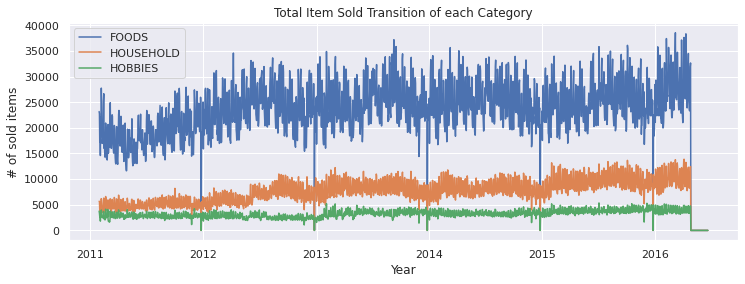
\includegraphics[width=0.8\linewidth]{img/meh.png}
  \end{center}
    \caption{Example of caption.  It is set in Roman so that mathematics
    (always set in Roman: $B \sin A = A \sin B$) may be included without an
    ugly clash.}
  \label{fig:long}
  \label{fig:onecol}
\end{figure}

\noindent
Compare the following:\\
\begin{tabular}{ll}
 \verb'$conf_a$' &  $conf_a$ \\
 \verb'$\mathit{conf}_a$' & $\mathit{conf}_a$
\end{tabular}\\
See The \TeX book, p165.

The space after \eg, meaning ``for example'', should not be a
sentence-ending space. So \eg is correct, {\em e.g.} is not.  The provided
\verb'\eg' macro takes care of this.

When citing a multi-author paper, you may save space by using ``et alia'',
shortened to ``\etal'' (not ``{\em et.\ al.}'' as ``{\em et}'' is a complete word.)

For this citation style, keep multiple citations in numerical (not
chronological) order, so prefer \cite{Alpher03,Alpher02,Authors06} to
\cite{Alpher02,Alpher03,Authors06}.





This is fractions text area is $6\frac78$ inches (17.5 cm) wide by $8\frac78$
and more $\frac{5}{16}$ and other $8.5 \times 11$-inch

Reference figurers Figures~\ref{fig:onecol} and~\ref{fig:short}.  Short captions should be centred.

\noindent For no indent

FIRST-ORDER HEADINGS. (For example, {\large \bf 1. Introduction})

SECOND-ORDER HEADINGS. (For example, { \bf 1.1. Database elements})

Please use footnotes\footnote {This is what a footnote looks like.  It
often distracts the reader from the main flow of the argument.} sparingly.

\begin{table}
  \begin{center}
    \begin{tabular}{|l|c|}
      \hline
      Method & Frobnability \\
      \hline\hline
      Theirs & Frumpy \\
      Yours & Frobbly \\
      Ours & Makes one's heart Frob\\
      \hline
    \end{tabular}
  \end{center}
  \caption{Results.   Ours is better.}
\end{table}

When placing figures in \LaTeX, it's almost always best to use
\verb+\includegraphics+, and to specify the  figure width as a multiple of
the line width as in the example below
{\small\begin{verbatim}
   \usepackage[dvips]{graphicx} ...
   \includegraphics[width=0.8\linewidth]
                   {myfile.eps}
\end{verbatim}
}


{\small
\bibliographystyle{ieee}
\bibliography{egbib}
}

\end{document}
